\documentclass[]{article}
\usepackage{graphicx}
\usepackage{amsmath}

\usepackage{authblk}

\makeatletter
\renewcommand \thesection{S\@arabic\c@section}
\renewcommand\thetable{S\@arabic\c@table}
\renewcommand \thefigure{S\@arabic\c@figure}
\makeatother


\usepackage[backend=bibtex, style=phys, articletitle=false,  biblabel=brackets, sorting=none]{biblatex}
\bibliography{chgcnn}

\DeclareFieldFormat{journaltitle}{\mkbibemph{#1}}
\DeclareFieldFormat{pages}{#1}


%opening

\title{Supplementary Information:\\ Crystal Hypergraph Convolutional Networks}
\author{
	Alexander J. Heilman$^{1}$, Weiyi Gong$^{1}$, and Qimin Yan\thanks{Corresponding Author: q.yan@northeastern.edu}$^{1}$
}

\affil{\textit{
		$^1$Department of Physics, Northeastern University, 
		Boston, MA 02115, USA}}
  
\date{}

\begin{document}

\maketitle

\section{Motif Features: Structure Order Parameters \& Continuous Symmetry Measures}
The geometry of the motifs were incorporated as features composed of a concatenated list of structure order parameters and continuous symmetry measures (CSMs) for a set of common local environments. 

Structure order parameters are coordinate system invariant measures of 3 dimensional structure that are designed to be close to one when a given structure is similar to some prototypical arrangement. Note that this isn't in general a true 'distance'-like measure to some shape as a CSM is, however. A CSM is essentially defined so that it may act as a 'distance' from some prototypical shape to some given structure. The list of order parameters included as motif features are those that implemented in existing pymatgen code and described in \cite{orderparam1, orderparam2}.


\section{CHGConv}\label{chgconv}
A specific implementation of a hypergraph convolutional operator in the hypergraph message passing framework is a generalization of CGConv implemented in pytorch geometric and based on CGCNN's convolutional operator defined in eq (5) of the original paper.

\begin{align*}
	x_i^{t+1} &= \sum_{b_j} f(x_i^t, b_j,\text{AGG}(\lbrace x_j^t\in b_j \rbrace )) \\ 
	& = \text{BN}\bigg[\sum_{b_j}\sigma \big(W_c\cdot [x_j\oplus b_j\oplus \text{AGG}(\lbrace x_j^t\in b_j \rbrace ] )\big)\\
	&\quad\quad\cdot S^+ (W_f\cdot (x_j\oplus b_j\oplus \text{AGG}(\lbrace x_j^t\in b_j \rbrace ) )  ) \bigg]
\end{align*}
For the model utilized in this work, the $\text{AGG}$ function chosen was a combined set of component-wise maximum, minimum, average, and standard deviation, all with learnable attention weights. This combined use of multiple aggregation functions was inspired by a similar approach taken in the \textit{ChemGNN} model \cite{chemgnn}.

\section{Hyperparameters for Testing}\label{app:hyperparam}
For each convolutional structure, testing was done for a model with 3 convolutional layers. Each convolutional layer consists of back-to-back convolution from the smallest to the largest hyperedge type (for example two bond \& motif layers consist of a total sequence of bond, motif, bond and motif convolution). 

\begin{center}
\begin{tabular}{|l|c|}
	\hline 
	\multicolumn{1}{|c|}{\textbf{Hyperparameter}} & \multicolumn{1}{c|}{\textbf{Value}} \\
	\hline
	Node Hidden Feature Dimension & 64 \\
	Post-Convolution Linear Width & 128\\
	Number of Convolutional Layers & 3\\
	Number of Epochs & 300 \\
	Batch-size & 16 ($< 20,000$ Samples) \textit{or} 64 \\
	Optimizer & SGD \\
	Learning Rate (Epoch $<$150) & 0.01\\
	Learning Rate (Epoch $>$150) & 0.001\\
	\hline
\end{tabular}
\end{center}

Stochastic gradient descent (SGD) was used as an optimizer through training with an initial learning rate of 0.01. A multi-step learning rate scheduler divided this learning rate by a factor of 10 at epoch 150, with training running for a total of 300 epochs.  

Hidden node features were of dimension 64 through all convolutional layers, and a hidden output layer of dimension 128 was used (similar to CGCNN's architecture). The loss functions utilized were Mean Squared Error (MSE, for regression tasks) and cross entropy (for classification tasks). Accuracy is then reported in Mean Absolute Error (MAE) for regression tasks and area under curve (AUC) for classification tasks. 

Results reported were averaged over 5 folds of nested cross-validation. The datasets were divided into 80\% for training and 20\% for test for each fold, with a further 20\% of the training subset being used as an indicative validation set, where the best performance on this dataset was used to select the model applied to the test set. 


\section{Comparison to Line Graph}
A more usual approach for the incorporation of bond angle information is via the construction of a line graph, as in \cite{alignn, m3gnet}. 
\begin{center}
	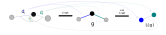
\includegraphics[scale=0.72]{line_graph_ex.pdf}
\end{center}
These models generally first update the edge features of the crystal graph $\mathcal{G}$ by first applying some graph convolutional operator to the line graph $L(\mathcal{G})$ with angles encoded in  $L(\mathcal{G})$'s initial edge features.

Our argument against such representation schemes here is that the order of messages grows combinatorically for derived line graphs as $\mathcal{O}(nm^2)$, where $n$ is the number of nodes and $m$ is the average number of edges per node in $\mathcal{G}$.

Here, we incorporate a similar level of higher-order geometrical structure instead in a local environment, or 'motif', hyperedge (defined below). Note that these include only an extra number of messages on the order $\mathcal{O}(mn)$ if each node in a motif gets a message, or on the order $\mathcal{O}(n)$ if only center nodes are updated by their own motif hyperedges.


\section{Hyperedge Index}
Hypergraphs are treated as a set of node feactures $x$, hyperedge features $h$, and hyperedge indices $I$. 
The hyperedge index is, computationally, treated as a $[2,nm]$ dimensional vector (where $m$ is the number of hyperedges and $n$ is the avereage number of nodes contained in any hyperedge). 
The first index is the node contained and the second index is the containing hyperedge (as in \cite{hypergraphconv}). This scheme is depicted in an example in Figure \ref{hyperedgeindex_fig}
\begin{figure}[!h]
\begin{center}
	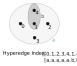
\includegraphics[scale = 0.8]{hyperedge_index.pdf}
\end{center}
\caption{Hyperedge index example for a specific hypergraph.}\label{hyperedgeindex_fig}
\end{figure}

\section{Message Number Scaling for Different Hyperedge Types}
The rationale for including motifs in lieu of triplets (as in line graphs) is most poignant when considering material systems of increasing unit-cell size. To make this point most clear, here we consider the number of hyperedges required for the three different types of hyperedges considered in this work for different sized supercells of Manganese Oxide (MnO$_2$) in Figure \ref{message_scaling_fig}.

\begin{figure}[!h]
\begin{center}
	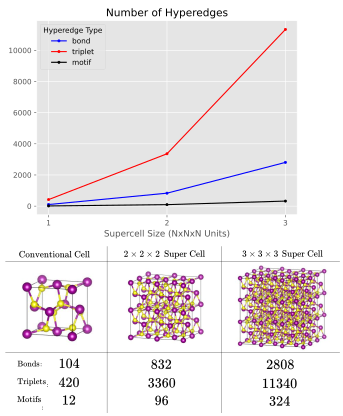
\includegraphics[scale=0.35]{message_scaling.pdf}
\end{center}
\caption{Figure tabulating the number of hyperedges of each type for increasing supercell size. The example material here is Manganese Oxide (MnO$_2$). }\label{message_scaling_fig}
\end{figure}

Here, the number of triplets clearly grows exponentially, whereas the number of bonds grows quadratically, and the number of motifs, linearly. As such, additional geometric resolution may be afforded by relatively few motif hyperedges, as compared to triplet-based constructions.


\section{Case Study on Discrimination of Similar Environments}
To demonstrate the importance of motif-level hyperedges in applications to material systems, the node embeddings of two compositionally-similar, but structurally distinct materials are considered here: Trigonal ($T$-phase) and Hexagonal ($H$-phase) MoS$_2$. To demonstrate the effectiveness of the motif models in sooner recognizing structural differences, the difference in these node embeddings are compared within these material sets through 300 epochs of training for models with 1 convolutional layer of either bond-, motif-, or triplet-level hyperedges. Node representation difference was calculated by subtracting the normalized dot-product of the central atom's node embeddings from one. This node representation difference through training is shown in Figure \ref{node_diff_fig}.

%\begin{figure}
%\begin{center}
%	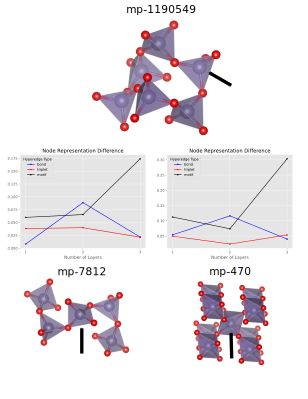
\includegraphics[scale=0.32]{similar_cells_GeO2.pdf}
%\end{center}
%\caption{Difference in node representations after 1-3 layers of either bond-, motif-, or triplet-only layers as determined by one minus the normalized dot product of central node representations for three crystalline phases of GeO$_2$. Note that the nodes under consideration are specified by bold black arrows overlayed on their material graphic. These material CIFs were taken from the Materials Project, and their corresponding MP-id is provided along with their graphic.}
%\end{figure}
While bond-only models could generally distinguish the node embeddings of central atoms between these different, but similar, structures, the motif-based model captured the structural differences earliest (that is, the one-layer models of motifs always show the greatest difference). Specifically, the motif-only model had a representation difference of 0.004 after 1 epoch of training, whereas the triplet and bond-only models had an initial difference of 0.0005 and 0.00025, respectively. After 300 epochs, the motif-only model still had the largest difference of 0.075, while the triplet model's difference had increased to 0.008 and the bond-only model had remained similar with a difference of 0.00029. This demonstrates that the motif-only model had the greatest discrimination between the two similar environments, a difference relevant to the band gap target since $H$-phase MoS$_2$ is insulating (with a band gap of zero), and $T$-phase  MoS$_2$ is not (with a band gap of 1.2 eV). However, it should be noted this metric is unreliable, insofar that neural networks are essentially black boxes and hence sheer differences in node embeddings are hard to translate directly to model performance. 
\begin{figure}[!h]
\begin{center}
	\includegraphics[scale=0.4]{MoS2_similar_cells_update2.pdf}
\end{center}
\caption{Normalized dot product difference between H-phase and T-phase MoS$_2$ central Molybdenum node representations across 300 epochs of 1 layer of either bond-, motif-, or triplet-only convolution. Here, red is the difference across epochs for the motif-only model; blue is for triplet-only model; and black represents the difference for the bond-only model.}\label{node_diff_fig}
\end{figure}


\section{Comparison of Order Parameters and Continuous Symmetry Measures as Motif Features}
To compare the importance of motif features, the data set that most benefited from motif features were tested both with and without the two primary types of motif features considered in this work: Local Structure Order Parameters (LSOPs) as defined in \cite{orderparam1, orderparam2}; and Continuous Symmetry Measures \cite{csm_polyhedra,coord_polyhedra} for 59 common coordination polyhedra. Bond and motif convolutional models were tested on this bulk moduli dataset for 500 epochs with no motif features, only CSMs, only LSOPs, and both feature sets concatenated. For all tests, the batch size was 128, Stochastic Gradient Descent was used as the optimizer with an initial learning rate of 0.1, with a reduced learning rate of 0.01 being applied at epoch 300. These results are tabulated in Table \ref{motiffeattable}.


\begin{table}[!h]
\begin{center}
\begin{tabular}{|c|c|}
	\hline
\textbf{Motif}	&\textbf{Validation MAE} \\
\textbf{Features} & $\text{Log}_{10}(K_{vrh})$\\
	\hline
	None & 0.0777 \\
	CSMs & 0.0758 \\
	LSOPs & 0.0785 \\
	Both &  0.0772 \\
	\hline
\end{tabular}
\end{center}
\caption{Table showing validation results for model performance on bulk moduli after 500 epochs of training. Note that here, distinct validation and test sets are not used. Instead model performance is tested once on the validation set after training, with a 90\% training / 10\% validation split of the total data set.}\label{motiffeattable}
\end{table}



CSM-only features performed best on the validation set, suggesting they have offer better generalizatbility as a feature. This may be due to the fact that CSM-based features result in sparse (similar to one-hot) encodings, whereas LSOP features tend more towards scalar-valued features. That is, while both CSMs and LSOPs are scalar-valued, a large subset of incommensurate ideal shapes used in CSM calculations results in many zero entries, whereas LSOPs may generally be computed regardless and just return smaller scalar values, so that the sparse CSM features may more adequately distinguish environments through the model.

\section{Performance on Matbench Folds}
Results tabulated in the main text are averaged over 5 folds of nested cross-validation, with test indexes supplied by MatBench \cite{matbench}. Accordingly, the uncertainty in test performance $\Delta x$ is calculated as:
\begin{equation}
\Delta x = \frac{R}{2\sqrt{N}}
\end{equation}
with $R$ the range of values and $N$ the number of runs (here, 5 for the 5 folds). Furthermore, the test set performance for each fold is tabulated below. Furthermore, in the following, $\bar{x}$ denotes the average of the values in the column above. These results are shown in Tables S2-S10 below.
\begin{table}
\begin{center}
	\begin{tabular}{|c|c|c|c|}
		\hline
		\multicolumn{4}{|c|}{Perovskite - Formation Energy} \\
			\multicolumn{4}{|c|}{Test MAE (meV/atom)}\\
		\hline
		Fold & Bond-only & Bond \& Motif & Bond \& Triplet\\
		\hline
		1 & 0.0436 & 0.0427 &0.0422 \\
		2 & 0.0441&0.0433&0.0427 \\
		3 & 0.0421&0.0420&0.0431 \\
		4 & 0.0429&0.0404&0.0423 \\
		5 & 0.0436&0.0430&0.0429\\
		\hline
		$\bar{x}$ &0.0433 &0.0423 & 0.0426 \\
		$\Delta x$ &4$\times$10$^{-4}$& 7$\times$10$^{-4}$& 2$\times$10$^{-4}$\\
		\hline
	\end{tabular}
\end{center}
\caption{Performance across the 5 MatBench test folds on the perovskite formation energy target set.}
\end{table}

\begin{table}
\begin{center}
	\begin{tabular}{|c|c|c|c|}
		\hline
		\multicolumn{4}{|c|}{Log$_{10}$(K$_{vrh}$)} \\
					\multicolumn{4}{|c|}{Test MAE  (Log$_{10}$GPa)}\\
		\hline
		Fold & Bond-only & Bond \& Motif & Bond \& Triplet\\
		\hline
		1 & 0.0669&0.0627 &0.0649 \\
		2 & 0.0682&0.0649&0.0669 \\
		3 & 0.0658&0.0613&0.0672 \\
		4 & 0.0710&0.0667&0.0680 \\
		5 & 0.0688&0.0623&0.0661\\
		\hline
		$\bar{x}$ &0.0681 &0.0636 & 0.0666 \\
		$\Delta x$ &1.2$\times$10$^{-3}$& 1.2$\times$10$^{-3}$& 0.7$\times$10$^{-3}$\\
		\hline
	\end{tabular}
\end{center}
\caption{Performance across the 5 MatBench test folds on the bulk moduli target set.}
\end{table}

\begin{table}
\begin{center}
	\begin{tabular}{|c|c|c|c|}
		\hline
		\multicolumn{4}{|c|}{Log$_{10}$(G$_{vrh}$) } \\
							\multicolumn{4}{|c|}{Test MAE  (Log$_{10}$GPa)}\\
		\hline
		Fold & Bond-only & Bond \& Motif & Bond \& Triplet\\
		\hline
		1 & 0.0839&0.0805 &0.0840 \\
		2 & 0.0848&0.0815&0.0866 \\
		3 & 0.0857&0.0817&0.0853 \\
		4 & 0.0825&0.0797&0.0825 \\
		5 & 0.0826&0.0813&0.0844\\
		\hline
		$\bar{x}$ &0.0839 &0.0809 & 0.0846 \\
		$\Delta x$ &7$\times$10$^{-4}$& 4$\times$10$^{-4}$& 9$\times$10$^{-4}$\\
		\hline
	\end{tabular}
\end{center}
\caption{Performance across the 5 MatBench test folds on the shear moduli target set.}
\end{table}

\begin{table}
\begin{center}
	\begin{tabular}{|c|c|c|c|}
		\hline
		\multicolumn{4}{|c|}{Highest Phonon Peak $\omega$ } \\
		\multicolumn{4}{|c|}{Test MAE  (cm$^{-1}$)}\\
		\hline
		Fold & Bond-only & Bond \& Motif & Bond \& Triplet\\
		\hline
		1 & 77.6& 59.7 & 79.8 \\
		2 & 50.6& 43.8 & 40.8 \\
		3 & 59.3& 55.3 & 63.7 \\
		4 & 49.6& 55.9 & 56.8 \\
		5 & 47.8& 50.0 & 62.4\\
		\hline
		$\bar{x}$ &57.0 &52.9 & 60.7 \\
		$\Delta x$ &6.7& 3.6& 8.7\\
		\hline
	\end{tabular}
\end{center}
\caption{Performance across the 5 MatBench test folds on the phonon peak target set.}
\end{table}

\begin{table}
\begin{center}
	\begin{tabular}{|c|c|c|c|}
		\hline
		\multicolumn{4}{|c|}{Dielectric Constant} \\
		\multicolumn{4}{|c|}{Test MAE}\\
		\hline
		Fold & Bond-only & Bond \& Motif & Bond \& Triplet\\
		\hline
		1 & 0.323 & 0.343 & 0.353 \\
		2 & 0.419& 0.419 & 0.380 \\
		3 & 0.575& 0.533 & 0.582 \\
		4 & 0.461& 0.447 & 0.476 \\
		5 & 0.464& 0.415 & 0.407\\
		\hline
				$\bar{x}$ &0.448 &0.431 & 0.440 \\
		$\Delta x$ &0.056 & 0.043 & 0.051\\
		\hline
	\end{tabular}
\end{center}
\caption{Performance across the 5 MatBench test folds on the dielectric constant target set.}
\end{table}

\begin{table}
\begin{center}
	\begin{tabular}{|c|c|c|c|}
		\hline
		\multicolumn{4}{|c|}{Exfoliation Energy (Jdft2d)} \\
		\multicolumn{4}{|c|}{Test MAE  (meV/Atom)}\\
		\hline
		Fold & Bond-only & Bond \& Motif & Bond \& Triplet\\
		\hline
		1 & 37.0 & 48.4 & 38.5 \\
		2 & 60.1& 44.8 & 57.4 \\
		3 & 78.3& 63.1 & 77.2 \\
		4 & 35.3& 30.4 & 64.6 \\
		5 & 58.0& 47.9 & 56.3\\
		\hline
		$\bar{x}$ &53.7&46.9& 58.8 \\
		$\Delta x$ &9.6& 7.3&8.7 \\
		\hline
	\end{tabular}
\end{center}
\caption{Performance across the 5 MatBench test folds on the exfoliation energy target set for a set of X 2D materials (labelled Jdft2d by MatBench).}
\end{table}

\begin{table}
\begin{center}
	\begin{tabular}{|c|c|c|}
		\hline
		\multicolumn{3}{|c|}{MP - Band Gap} \\
		\multicolumn{3}{|c|}{Test MAE (meV)}\\
		\hline
		Fold & Bond-only & Bond \& Motif \\
		\hline
		1 & 0.250 & 0.239 \\
		2 & 0.252 & 0.229 \\
		3 & 0.254 & 0.226 \\
		4 & 0.284 & 0.222 \\
		5 & 0.257 & 0.239 \\
		\hline
		$\bar{x}$ &0.259
		 &0.231 \\
		$\Delta x$ & 0.008 & 0.004 \\
		\hline
	\end{tabular}
\end{center}
\caption{Performance across the 5 MatBench test folds on the Materials Project band gap target set.}
\end{table}

\begin{table}
\begin{center}
	\begin{tabular}{|c|c|c|}
		\hline
		\multicolumn{3}{|c|}{MP - Formation Energy} \\
		\multicolumn{3}{|c|}{Test MAE (meV/atom)}\\
		\hline
		Fold & Bond-only & Bond \& Motif \\
		\hline
		1 & 0.0368&0.0347 \\
		2 & 0.0377&0.0402 \\
		3 & 0.0367&0.0369 \\
		4 & 0.0380&0.0498 \\
		5 & 0.0371&0.0370 \\
		\hline
		$\bar{x}$ &0.0373&0.0397 \\
		$\Delta x$ & 0.3$\times$10$^{-3}$&3.4 $\times$10$^{-3}$\\
		\hline
	\end{tabular}
\end{center}
\caption{Performance across the 5 MatBench test folds on the Materials Project formation energy target set.}
\end{table}

\begin{table}
\begin{center}
	\begin{tabular}{|c|c|c|}
		\hline
		\multicolumn{3}{|c|}{MP - Metalicity} \\
		\multicolumn{3}{|c|}{Test AUC}\\
		\hline
		Fold & Bond-only & Bond \& Motif\\
		\hline
		1 & .957& .960 \\
		2 & .951& .957 \\
		3 & .953& .958 \\
		4 & .955& .960 \\
		5 & .954& .955 \\
		\hline
		$\bar{x}$ &0.954&0.958 \\
		$\Delta x$ & 1.3$\times$10$^{-3}$&1.2 $\times$10$^{-3}$\\
		\hline
		\end{tabular}
\end{center}
\caption{Performance across the 5 MatBench test folds on the Materials Project metallicity target set.}
\end{table}

\printbibliography 

\end{document}
